\subsubsection{Radon profile classification}


\cite{2018MNRAS.480.2217S} identified 5 commonly recurring patterns in the stellar and gas Radon profiles of their MaNGA sample. These patterns were used to classify the Radon profiles observed in their MaNGA sample. In this work we adopt the same classification approach for the Radon profiles of the PSB galaxies and their control samples. Simplified models of 4 of the classes are shown in Figure \ref{fig:class-models}. In addition an asymmetric profile class was identified. The salient features of the Radon profile classes are listed below:

\begin{itemize}
    \item Constant, \textbf{Type-C} : Radon profile with relatively constant trace minimum angle $\hat{\theta}$ at all radii $\rho$.
    \item Inner Bend, textbf{Type-IB} : Galaxies whose Radon profiles exhibit symmetrical variations of $\hat{\theta}$ beginning at $|\rho|=0$, then transitioning to a constant value. 
    \item Outer Bend, \textbf{Type-OB} : Galaxies with constant Radon trace angle $\hat{\theta}$  at small $|\rho|$ which transition to a different value at a greater radius. 
    \item Inner Bend + Outer Bend, \textbf{Type-IB+OB} : Galaxies with Radon profiles showing a combination of the features of Type-IB and Type OB profiles.
    \item Asymmetric, \textbf{Type-A} : The value of the $\hat{\theta}$ varies significantly with $\rho$ across opposite sides of the transform R\textsubscript{AB}. 
 \end{itemize}

\begin{figure}
    \centering
    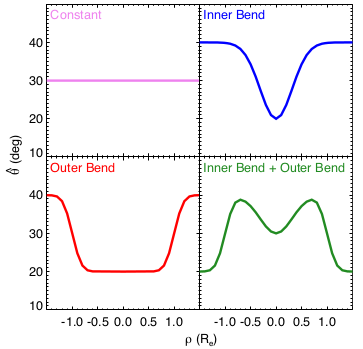
\includegraphics[width=\columnwidth]{images/RadonPlots/Radon-class-models.png}
    \caption{Toy model Radon transform examples of four of the RT classes used for visual classification of the RT trace plots. upper left: Constant, Type-C, upper right: Inner Bend, Type-IB, lower left: Outer Bend, Type-OB, and lower right: inner bend + outer bend, Type-IB+OB. Figure 8 from Stark et al. (2018).}
    \label{fig:class-models}
\end{figure}

Mathematical functions describing these Radon profile classifications have been identified by \citet[][section 3.6]{2018MNRAS.480.2217S}. This has enabled the development of code routines to provide automatic classification of the Radon trace profiles for galaxies in MaNGA Product Launch MPL-5. 

We don not presently have access to the automatic Radon trace classification code developed by \citet[][]{2018MNRAS.480.2217S}, so for this work we adopt a simple visual classification method to categorise our sample galaxy into one of the 5 Radon profile trace types listed above. The visual classification process is described as follows. Firstly we obtain the MAPS datacube FITS files for the selected PSB galaxies listed in Tables \ref{tab:my-CPSBs} and \ref{tab:my-RPSBs}, and a similar number of 'normal' galaxies drawn from their respective control samples, as described in Section  \ref{sec:controls}, downloaded via the MaNGA Marvin web interface. We then process each of datacubes through the Radon transform wrapper code to obtain PostScript output files showing the galaxy SDSS $gri$ image cutout, the MaNGA stellar velocity map, the absolute bounded Radon transform R\textsubscript{AB} plot and the Radon profile plot of $\hat{\sigma}$ versus $\rho$. An example of this output is shown in Figure \ref{fig:RT-CPSB-9493-12705-SNIP}. Next we examine the output plot for each galaxy and visually assess the qualitative strength of each of the 5 classification features by assigning a numeric weighting as given in Table \ref{tab:features}.

\begin{table}
    \centering
    \begin{tabular}{cl}
    \hline
    Value & Visual appearance \\
    \hline
    2 & Feature strongly apparent \\
    1 & Some evidence of feature \\
    0 & Feature absent \\
    \hline
    \end{tabular}
    \caption{Relative weighting of Radon profile feature strengths used for visual classification of Radon profile feature types: Constant, Inner Bend, Outer Bend, Inner Bend + Outer Bend or Asymmetric.}
    \label{tab:features}
\end{table}